\section{Ideale}

Sei $R$ ein Ring. (Die meisten Beweise finden sich wieder im LAAG 1+2 Skript!)

\begin{definition}[Ideal]
	Ein \begriff{Ideal} von $R$ ist eine Untergruppe $I \leq (R,+)$ mit $a \in I$, $r \in R \to ra \in I$ (in Zeichen: $I \unlhd R$).
\end{definition}

\begin{example}
	\begin{enumerate}[label=(\alph*)]
		\item Für $a \in R$ ist $(a) := Ra = \{ra \mid r \in R\}$ das von $a$ erzeugte \begriff{Hauptideal}.
		\item $(0)$ das \begriff[Ideal!]{Nullideal}
		\item $(1) = R$ das \begriff[Ideal!]{triviale Ideal} (ein Ideal $I \unlhd R$ mit $I \neq R$ ist ein \begriff[Ideal!]{echtes Ideal}  von $R$) 
	\end{enumerate}
\end{example}

\begin{remark}
	\proplbl{2_2_3}
	\begin{enumerate}[label=(\alph*)]
		\item $I \subseteq R$ ist Ideal von $R \Leftrightarrow I + I \subseteq$, $R \cdot I \subseteq I$, $0 \in I$
		\item Ein Ideal von $R$ ist im Allgemeinen kein Unterring von $R$.
		\item Für $I \unlhd R$ ist $I = R \Leftrightarrow 1 \in I$
		\item Für ein $a \in R$ gilt: $(a) = R \Leftrightarrow a \in R^{\times}$\\
		Insbesondere gilt: Genau dann ist $R$ ein Körper, wenn $(0) \neq (1)$ die beiden einzigen Ideale von $R$ sind.
		\item Sind $I,J \unlhd R$, so auch $I + J$ und $I \cap J$.
		\item Der Schnitt einer Familie $(I_\lambda)_{\lambda \in \Lambda}$ von Idealen von $R$ ist wieder ein Ideal von $R$. Insbesondere existiert zu jedem $A \subseteq R$ ein kleinstes Ideal $\langle A \rangle$ von $R$, das $A$ enthält (das von $A$ \begriff{erzeugte Ideal}). Es gilt
		\begin{align}
			\langle A \rangle = \left\{ \sum_{i=1}^{n} r_i a_i \mid n \in \natur, r \in R, a_i \in A\right\} \notag
		\end{align}
	\end{enumerate}
	Wir schreiben $(a_1, \dots, a_n)$ für $\langle\{ a_1, \dots, a_n \}\rangle$.
\end{remark}

\begin{example}
	Ist $\phi: R \to S$ ein Ringhomomorphismus, so ist $\Ker(\phi) \unlhd R$: $\phi(a) = 0$,$ \phi(b) = 0$ \\
	$\Rightarrow \phi(a+b) = \phi(a) + \phi(b) = 0$\\
	$\Rightarrow \phi(ra) = \phi(r)\cdot \phi(a) = 0$
\end{example}

\begin{definition}[Quotientenring] 
	Sei $I \unlhd R$. Der \begriff{Quotientenring} (QR) von $R$ modulo $I$ ist
	\begin{align}
		\lnkset{R}{I} = \{x+i\mid x\in R\}\notag
	\end{align}
	mit $x, y \in R$
	\begin{itemize}
		\item $(x+ I) +_{QR} (y+I) := (x+y) +I$
		\item $(x+I) \cdot_{QR} (y+I) := (xy) +I$
	\end{itemize}
\end{definition}

\begin{proposition}
	\proplbl{2_2_6}
	$\lnkset{R}{I}$ ist ein Ring und $\pi_I : R \to \lnkset{R}{I}$ mit $x \mapsto x +I$ ist ein Ringhomorphismus mit Kern $I$.
\end{proposition}
\begin{proof}
	Siehe LAAG VIII.5.8.
\end{proof}

\begin{remark}
	\begin{enumerate}[label=(\alph*)]
		\item Die Ideale sind also genau die Kerne von Ringhomomorphismen.
		\item Für $x,y \in R$ schreibt man
		\begin{align}
			x \equiv y \mod I &\Leftrightarrow x - y \in I\notag \\
			&\Leftrightarrow x+I = y+I\notag \\
			&\Leftrightarrow \pi_I(x) = \pi_I(y) \notag
		\end{align}
	\end{enumerate}
\end{remark}

\begin{proposition}[Homomorphiesatz]
	\proplbl{2_2_8}
	Sei $\phi: R \to S$ ein Ringhomomorphismus und $I \unlhd R$ ein Ideal mit $I \subseteq \Ker(\phi)$. Dann gibt es genau einen Ringhomomorphismus $\overline{\phi}:\lnkset{R}{I} \to S$ mit $\phi = \overline{\phi}\circ \pi_I$
		\begin{center}
		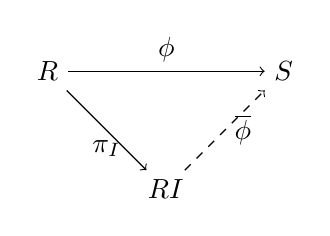
\begin{tikzpicture}
		\node (M) at (0,0) {$R$};
		\node (MS) at (3,0) {$S$};
		\node (Q) at (1.5,-1.5) {$\lnkset{R}{I}$};
		\draw[->, above] (M) to node {$\phi$} (MS);
		\draw[->, below] (M)  to node {$\pi_I$} (Q);
		\draw[->, right, dashed] (Q)  to node {$\overline{\phi}$} (MS);
		\end{tikzpicture}
	\end{center}
	Insbesondere gilt: Ist $\phi$ surjektiv, so induziert $\phi$ ein Isomorphismus
	\begin{align}
		\lnkset{R}{\Ker(\phi)} \cong S. \notag
	\end{align}
\end{proposition}
\begin{proof}
	Siehe LAAG VIII.5.9.
\end{proof}

\begin{lemma}
	\proplbl{2_2_9}
	Sei $\phi:R\to S$ ein Ringhomomorphismus.
	\begin{enumerate}[label=(\alph*)]
		\item Für $J \unlhd S$ ist $\phi^{-1}(J) \unlhd R$.
		\item Ist $\phi$ surjektiv, so liefert $J \mapsto \phi^{-1}(J)$ eine Bijektion $\Phi$ zwischen
		\begin{enumerate}
			\item Idealen von $S$, und
			\item Idealen von $R$, die $\Ker(\phi)$ enthalten
		\end{enumerate}
	\end{enumerate}
\end{lemma}
\begin{proof}
	(vgl. LAAG VIII.5.5) Skizze:
	\begin{enumerate}[label=(\alph*)]
		\item $a \in \phi^{-1}(J)$, $r \in R$ $\Rightarrow \phi(ra) = \underbrace{\phi(r)}_{\in S}\underbrace{\phi(a)}_{\in J}\in J$
		\item Umkehrabbildung: $I \mapsto \phi(I)$
		\begin{itemize}
			\item $\phi(\phi^{-1}(J))=J\colon \phi$ surjektiv
			\item $\phi^{-1}(\phi(I)) = I\colon$ \propref{1_3_7}
			\item $I \unlhd R \Rightarrow \phi(I) \unlhd S: a \in I$, $s \in S \xRightarrow{\phi \text{ surjektiv}} s = \phi(r)$ mit $r \in R$:\\
			$\Rightarrow s \phi(a) = \phi(r)\phi(a) = \phi(ra)$ mit $ra \in I \Rightarrow s\phi(a) \in \phi(I)$
		\end{itemize}
	\end{enumerate}
\end{proof}

\begin{definition}[Primideal und maximales Ideal]
	Sei $I\unlhd R$.
	\begin{enumerate}[label=(\alph*)]
		\item $I$ ist \begriff[Ideal!]{prim} $:\Leftrightarrow I \neq R$ und für $a,b \in R$ gilt:
		\begin{align}
			ab \in I \Rightarrow a \in I \vee b \in I\notag
		\end{align}
		\item $I$ ist \begriff[Ideal!]{maximal} $:\Leftrightarrow I \neq R$ und ist $J \unlhd R$ mit $I \subseteq J \subsetneq R$, so ist $I=J$.
	\end{enumerate}
\end{definition}

\begin{proposition}
	\proplbl{2_2_11}
	Sei $I \properideal R$
	\begin{enumerate}[label=(\alph*)]
		\item $I$ ist prim $\Leftrightarrow \lnkset{R}{I}$ ist nullteilerfrei
		\item $I$ ist maximal $\Leftrightarrow \lnkset{R}{I}$ ist Körper
		\item $I$ ist maximal $\Rightarrow I$ prim
	\end{enumerate}
\end{proposition}
\begin{proof} 
	\begin{enumerate}[label=(\alph*)]
		\item Beachte: $\pi_I(a)=0 \Leftrightarrow a \in I$
		\begin{itemize}
			\item Hinrichtung: $a,b \in R$, $\pi_I(a)\cdot\pi_I(b) = 0\Rightarrow\pi_I(ab)=0$\\
			$\Rightarrow ab \in I \xRightarrow{I \text{ prim}} a \in I \vee b \in I\Rightarrow \pi_I(a) = 0 \vee \pi_I(b) = 0$
			\item Rückrichtung: $I$ nicht prim $\Rightarrow$ es existieren $a,b \in R$ mit $ab \in I$, $a \not\in I$, $b \not \in I\Rightarrow$ $0 = \pi_I(ab) = \underbrace{\pi_I(a)}_{\neq 0}\underbrace{\pi_I(n)}_{\neq 0}$\\
			$\Rightarrow \lnkset{R}{I}$ ist nicht nullteilerfrei
		\end{itemize}
		\item $I$ maximal $\xLeftrightarrow{\propref{2_2_9}b)} \lnkset{R}{I}$ hat nur die Ideale $(0) = \pi_I(1)$ und $(1) = \pi_I(R)$ $\xLeftrightarrow{\propref{2_2_3}d)}\lnkset{R}{I}$ ist Körper
		\item folgt aus a) und b), denn Körper sind nullteilerfrei!
	\end{enumerate}
\end{proof}

\begin{example}[Gegenbeispiel, dass die Umkehrung von \propref{2_2_11}c) nicht gilt!]
	In $R = \whole$: Ideale sind genau die Hauptideale
	\begin{align}
		(n) = n\whole,\quad n \in \natur_0\notag
	\end{align}
	\begin{itemize}
		\item $(n)$ ist prim $\Leftrightarrow n$ Primzahl oder $n = 0$
		\item $(n)$ ist maximal $\Leftrightarrow n$ Primzahl
	\end{itemize}
\end{example}

\begin{proposition}
	\proplbl{2_2_13}
	Jedes echte Ideal $I \properideal R$ ist in einem maximalen Ideal von $R$ enthalten.
\end{proposition}
\begin{proof}
	Sei $\mathcal{H} = \{ J \properideal R \mid I \subseteq J\}$. Wir wenden das Lemma von \person{Zorn} auf die Halbordnung $(\mathcal{H},\subseteq)$ an:
	\begin{itemize}
		\item $\mathcal{H} \neq 0$: $I \in \mathcal{H}$.
		\item Sei $(J_{\lambda})_{\lambda \in \Lambda}$ eine nichtleere Kette in $\mathcal{H}$. Dann ist $J = \bigcup J_{\lambda} \in \mathcal{H}$ eine obere Schranke für $(J_{\lambda})$:
		\begin{itemize}
			\item $I \subseteq J$: klar, da $I \subseteq J_{\lambda}$ für ein $\lambda \in \Lambda$
			\item $J \unlhd R$: Sind $a,a' \in J$, $r \in R$, so ist $a \in J_{\lambda}$ und $a' \in J_{\lambda'}$ für $\lambda, \lambda' \in \Lambda$. Da $\Lambda$ eine Kette ist, folgt dass (ohne Einschränkung) $J_{\lambda'} \subseteq J_{\lambda}$. Also $a+a' \in J_{\lambda} + J_{\lambda'} \subseteq J_{\lambda} \subseteq J$ und $ra \in R: J_{\lambda} \subseteq J$
			\item $J \neq R$: $J_{\lambda} \neq R$ für alle $\lambda \in \Lambda$. Also liegt die $1$ nicht in $J_{\lambda}$, also die $1$ auch nicht in $\bigcup J_{\lambda} = J$, d.h. $J \neq R.$
		\end{itemize}
	\end{itemize}
	Nach dem Lemma von \person{Zorn} hat $\mathcal{H}$ ein maximales Element $J$, das auch ein maximales Ideal ist.
\end{proof}

\begin{erinnerung}[Lemma von \person{Zorn}]
	Sei $(X,\le)$ eine Halbordnung, die nicht leer ist. Wenn jede Kette eine obere Schranke hat, dann hat $X$ ein maximales Element.
\end{erinnerung}

